\definecolor{lightgray}{rgb}{.9,.9,.9}
\definecolor{darkgray}{rgb}{.4,.4,.4}
\definecolor{purple}{rgb}{0.65, 0.12, 0.82}

\lstdefinelanguage{JavaScript}{
  keywords={typeof, new, true, false, catch, function, return, null, catch, switch, var, if, in, while, do, else, case, break},
  keywordstyle=\color{blue}\bfseries,
  ndkeywords={class, export, boolean, throw, implements, import, this},
  ndkeywordstyle=\color{darkgray}\bfseries,
  identifierstyle=\color{black},
  sensitive=false,
  comment=[l]{//},
  morecomment=[s]{/*}{*/},
  commentstyle=\color{purple}\ttfamily,
  stringstyle=\color{red}\ttfamily,
  morestring=[b]',
  morestring=[b]"
}

\lstset{
   language=JavaScript,
   backgroundcolor=\color{lightgray},
   extendedchars=true,
   basicstyle=\footnotesize\ttfamily,
   showstringspaces=false,
   showspaces=false,
   numbers=left,
   numberstyle=\footnotesize,
   numbersep=9pt,
   tabsize=2,
   breaklines=true,
   showtabs=false,
   captionpos=b
}



\chapter{Evaluation}

\section{Evaluation}
The previous chapters outlined our approach to feature extraction and visualization and demonstrated an implementation of that approach. The following chapters will evaluate the solution from a technical standpoint and from a subjective? standpoint taking into consideration the three main use cases that were presented initially.
\section{Technical Evaluation / Performance Evaluation}
\section{Case study: Network Administrator}
Let us suppose that a network operator has the task of investigating and reporting on a DDoS attack of which his infrastructure was the target. His objective would be to get a better idea of which types of attacks have happened and to create appropriate material to demonstrate what happened to and audience that could even be less technically proficient as him. We will assume for this scenario that the operator has a PCAP file of the attack and that the attack that was carried out with a multivector attack consisting of a portscan and a SYN-flood attack.

Since the user already has the PCAP file available and he aims at sharing the file only internally he can does not have to do the preprocessing steps as described with the researcher case study. Instead he will simply supply the name, description and PCAP file and start the upload process. Since this input contains real network traffic we suspect that this input file can be multiple megabytes or gigabytes of size. Both the analysis as well as the uploading procedure have been implemented to scale even for large file sizes, which means that one could run the application locally without requiring powerful hardware. Once the upload and analysis have finished the user receives a desktop notification, which allows the user to do other things without having to keep an eye on a loading spinner.
Now that the analysis file has finished the user will see some basic network state metrics right away. This is an important generalization which can serve for the reporting task. For example, he could directly see the number of destination ports that were targeted. In a very simple report he could list this number and suggest an appropriate solution, such as for example the adoption of a DMZ. Marty describes that network security professionel often have only minutes to present their subject to non-technical audiences \cite{appliedsecurityvisualization}. So reducing the incident to easily understandable facts is an important feature.
If the user desires to dig deeper into the patterns of the possible attacks he will open the dataset on the dashboard page. He may do this for one or more datasets so that he can build up a story where he would compare different traffic behaviours to underline his story. On the dashboard page he will find an item for each dataset which contains a visualization grouped by attack type. This grouping allows to observe the dataset under different perspectives which were written for specific attack behaviours. This allows to identify the attack vector, ie which attacks have been executed on the target. No make it easier to differentiate normal traffic from traffic behaviour under attack one can contrast the diagrams by opening the same diagram type using a different dataset. For example, in figure \ref{fig:datasettilesop} we can see a dataset of normal traffic and a dataset of traffic including attack rendered using the same feature extraction and the same graph. As one can see, the destination ports on the left side show that a large number of ports has received traffic compared to the right handside.
From this, the operator could draw an action such as a different configuration of a firewall. To support this proposal he could save the dashboard he just created and pull it up once he needs to make his proposal to an executive. For reporting purposes the user may also export a single diagram as PNG or the whole setup as PDF. This functionality is described in the "Eduction" case study.

\begin{figure}[datasettiles]
    \centering
    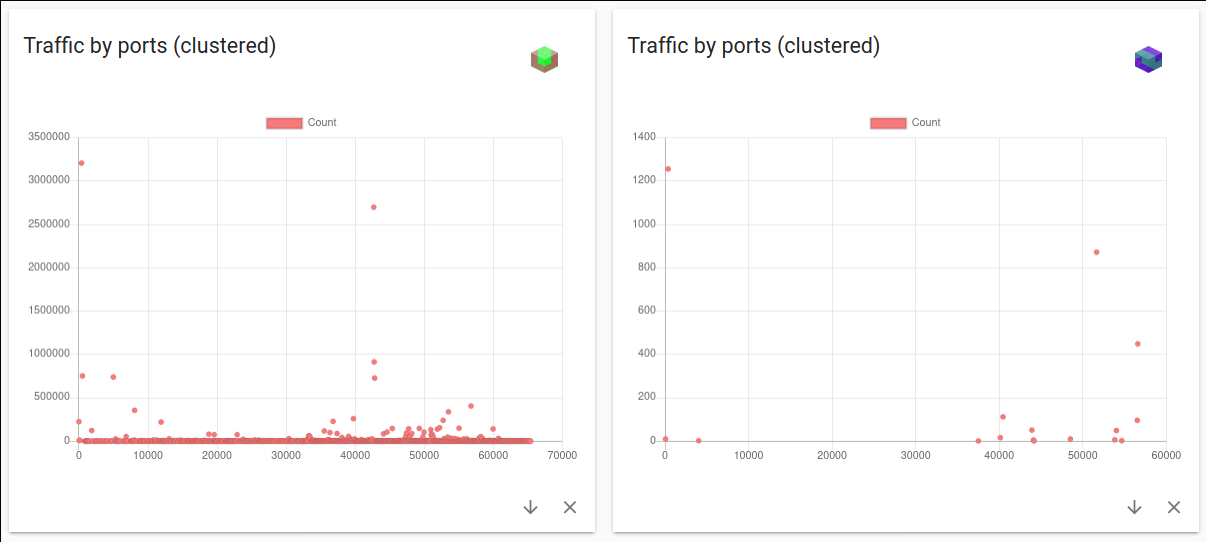
\includegraphics[width=15cm]{images/evaluation_different_datasets_same_visualization.png}
    \caption{Features from two datasets rendered on the same chart.}
    \label{fig:datasettilesop}
\end{figure}

We think that visualizations like this make it easy to simplify a picture of an attack, however this has to be taken with caution. Rendering destination ports can lead to common problem when visualizing network security-related incidents, namely the source-destinatino confusion described by Marty\cite{appliedsecurityvisualization}. The destination ports could be from incoming or outgoing packets which would distort the picture since incoming TCP packets of established connections will seem to have a random destination port, since it was picket by the targeted host. Our solution could help with this issue since the actual visualization is written by someone who would likely understand this attack pattern. It would be easy to integrate a warning message or propose a solution. The solution would to the actual problem would be to filter only the incoming packets not in established state, which can done during the capturing stage or later when performing the analysis. We have implemented a prototypical implementation that proves that it would be even possible to apply such a filter directly in our application. This would allow for a nice complementation of using tcpdump or wireshark to do initial pre-processing where one usually works with filters. The filters used initially could then be used in our application so that our application would be used solely for the reporting and creation of visualizations.


\section{Case study: Education}
Let us suppose that a professor in an educational facility wants to efficiently communicate the behaviour of an attack by visualizing its attack pattern. For this scenario, we will focus on one DDoS attack namel a SYN flood attack where a host is flooded with TCP connection requests that may stem from a spoofed source. (does this need a source?)
Existing network capture files from actual denial of service attacks might contain too much noise or might contain a multi-vector attack which could hinder the objective of explaining one specific attack dynamic. In this case the professor can obtain a networ capture by either performing an actual attack in a laboratory environment or he can use a tool such as DDoS\_log\_sim (TODO reference) to generate a network capture with the desired noise level. As output medium he would use the PCAP file format which is supported by our application. This is a common file format and supported by popular tools such as tcpdump and Wireshark.
Now that the capture file is available the professor can upload that file using the Datasets page of our application. He would do so by clicking the plus button in the lower right corner and supplying additional information such as a name and description which will be persisted as well. This is easy to work with since the professor could leave all network captures stored on the server and still distinguish between them by reading the description and names. For example, he could upload another capture file with a different attack pattern for a different audience and he could easily distinguish between them. This is also supported by generating an avatar from the MD5 hash of the file content. This makes it easy to distinguish between datasets just by glancing at the icon. Once the file is uploaded and the analysis is performed the user will be notified of a successfull completion through a desktop notification. Now he could open that dataset on the visualizations page or he could upload another dataset if he wants to show how that attack pattern looks with different parameters, for example one without any attack at all to show the difference in how the network dynamics appear.
Once he added all the datasets to the visualizations page he can transition to that page and create visualizations for each attack type he is interested in. The visualizations that are available for some dataset have been written for a specific attack although they can of course be used if an attack is not present. This grouping into attack categories should make it as easy as possible to open the right visualizations. This as well as the generated avatar and dataset names are shown in figure \ref{fig:datasettiles}

\begin{figure}[datasettiles]
    \centering
    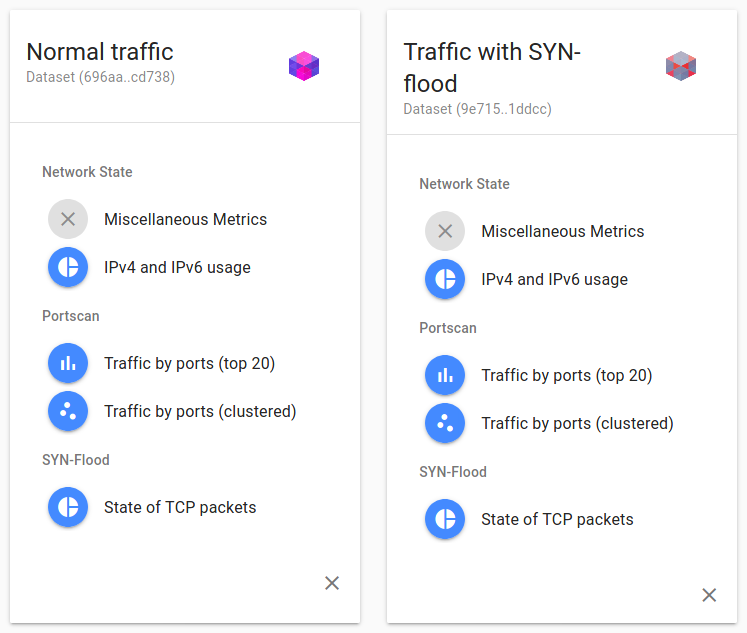
\includegraphics[width=13cm]{images/evaluation-dataset-tiles.png}
    \caption{Two different datasets opened on the visualizations page.}
    \label{fig:datasettiles}
\end{figure}
Since we defined that the professor in this scenario would be interested in a SYN-flood visualization he would open the piechart that was designed for this type of attack. This will create a new tile that briefly explains what is being displayed using a title and a legend (??). This tile will show the same avatar as the datasets tile to make it easier to understand to which dataset this visualization belongs. Using this visualization the professor can easily show that a large number of packets are in the (active) connection setup state of a TCP connection which clearly shows the attack pattern of a SYN flood state. This can be seen in figure \ref{fig:synfloodpiechart}. Now that the professor has a visualization of the attack pattern he could contrast this by either showing the same visualization for different traffic or showing a different visualization for the same dataset. This way he could contrast the attack with normal behaviour, which will make it clear that this is sometimes not a trivial task. It will also serve to show that there are no other attacks and that it is in fact a SYN-flood attack.

\begin{figure}[]
    \centering
    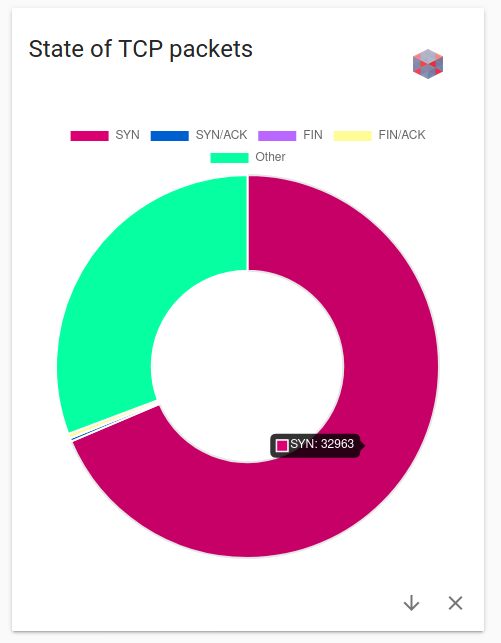
\includegraphics[width=10cm]{images/evaluation-synflood-piechart.png}
    \caption{Piechart showing the state of the TCP connection for each packet using a dataset that clearly contained a SYN-flood attack}
    \label{fig:synfloodpiechart}
\end{figure}
The professor can open new visualizations for the same or different datasets and close them again until he is satisfied with the dashboard and what he wants to present. Once this is the case he can decide how he wants to use the tool during presentation. First, he could save this setup in his browser cache and load it up at later stage. This would allow for all the interactivity that the visualizations provide, for example showing the actual number of packets in "SYN" state as shown in figure \ref{fig:synfloodpiechart}. This can be done by saving the dashboard in the lower right corner, where he may name the dashboard and then save it. This option is interesting because it remains the interactivity of our solution. This could be leveraged to let students play around with a dataset that was previously saved to a dashboard and find out on their own what type of attack might be contained.
Secondly he could export each visualization by clicking the arrow button on each tile. This will download it as a static PNG with a transparent background so that it could be used for presentations.
The last option would be to generate a PDF based on the dashboard that was created and download it.
We can compare our solution to the visualization feature of WireShark which we deem to be a popular alternative.
As one can see in figure \ref{fig:synvisualizationwireshark} it is absolutely possible to plot the same dataset using solely WireShark. However there are a few key differences. First off the IO-Graph from WireShark only gives the possibility to plot packets using time on the x-axis and frequency on the y-axis. It is however possible to have different lines for different filters and to configure the line styles. In any case, the filters need to be written manually, for example we would write a filter like "tcp.flags == 0x02" to show the packets in connection setup state. We would need to do this analogous for each other state, which can be cumbersome and which requires knowledge about the protocols implementation. With our solution the user of the tool could get to a similar graph without having to know about how the connection states are actually implemented in the protocol. Also, the fact that WireShark plots over time may be too detailed to actually get an abstract picture of the attack pattern. This can be improved by increasing the interval for each step on the x-axis.
Once one is satisfied with the configuration of the IO-Graph by supplying filters, colors, scaling and time interval one can view, modify and export the graph as a PDF. We think that these are all properties that hold for our solution as well, however with our solution one could save this setup for later usage and compare it with other datasets or with other graphs. Nevertheless, WireShark provides interesting features that would be beneficial to apply to our solution as well. This would cover the interactive scaling of the graph, changing the interval, dynamically adjusting colors and a graph that plots frequency over time. We deem that all of these features would be technically feasible to implement using our approach.

\begin{figure}[]
    \centering
    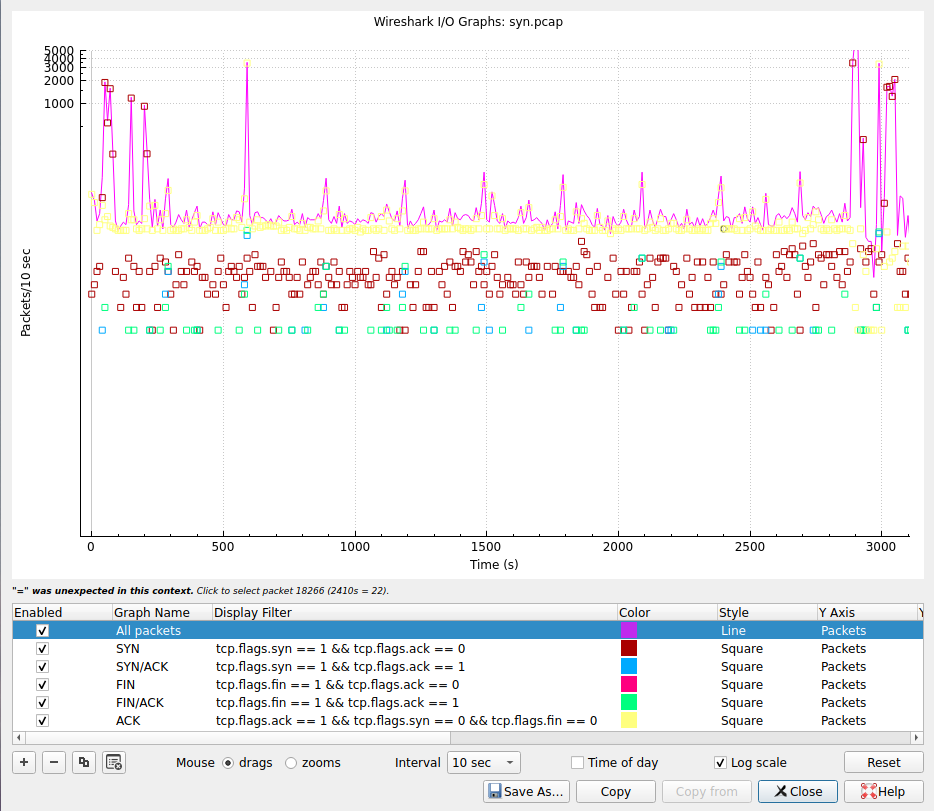
\includegraphics[width=13cm]{images/evaluation_wireshark_iograph_synflood.png}
    \caption{Plotting the same dataset using WireShark IO Graph with custom filters}
    \label{fig:synfloodpiechart}
\end{figure}

\section{Case study: Researcher}
So far we have explored cases that were able to use the existing functionality that was part of the prototypical implementation of our platform and feature extraction modules. Now we will focus on a case where this is not the case so that we will be able to focus on how the solution can be used as a platform for extension.
There could be many use-cases for example when a researcher has the task of computing a metric that is not yet computed with our feature extractors or when he wants to analyse a completely novel type of DDoS attack. We will assume that there is a researcher who has already analysed and explored the attack vector of his capture file but now he wants to derive other information by looking at different dimensions of the dataset. Specifically he would like to see which sources contributed the most packets to the inbound traffic. Thus he turns to our tool to implement his own feature extractor which will tell him the top five sources that were most often the source address of an IPv4 packet. Ideally, he would also like to supplement this information by enriching with sources other than the actual capture file. For example, he could use a BGP routing table to derive the prefix that the source IPv4 address belonged to.
So initially he will duplicate the template of a feature extractor and register it in the interface of the miner package. To do so, he will create a new file \textit{miner/miners/TopNSourceHostsByTraffic.js} with the content as shown in Listing \ref{lst:initialtemplate}.
Initially we just have a class that inherits from an abstract miner class which contains many convenience methods, for example for the writing of JSON files and the signaling of these files. It receives as dependency injection a packet decoder from which one may observe different packets. These subscriptions should be created in a \textit{setUp} method where one may perform asynchronous operations such as for example connecting to a database. The last method that will be called once all packets have been decoded is the \textit{postParsingAnalysis} which is again asynchronous to allow for asynchronous operations once all packets have been decoded. We will make use of this feature in the next step. At the end of that method the miner class should call the method of the base class that makes sure that the file is written and that everything is being orchestrated correctly. We can also see that the based on the structure of the final result the appropriate visualization will be used.


\begin{lstlisting}[caption={Initial content of the newly create Miner},float=H,label={lst:initialtemplate}]
const AbstractPcapAnalyser = require('./AbstractPCAPAnalyser')
const analysisName = 'TBD'

class SourceHostsAnalyser extends AbstractPcapAnalyser {
    constructor(parser, outPath) {
        super(parser, outPath);
        this.results = [
          // store interim results here
        ]
    }

    // Setup phase, load additional databases, setup subscriptions and signal completion
    async setUp() {
    }

    // Actual mining function
    // Post-analysis phase, do additional computation with the collected data and write it out
    async postParsingAnalysis() {

        var fileName = `${this.baseOutPath}-${analysisName}.json`
        var fileContent = {
          // Signal and format to visualize as piechart
          piechart: {
            datasets: [{
              backgroundColor: [],
              data: Object.values(this.results)
            }],
            labels: []
          }
        }
        var summary = {
            fileName: fileName,
            attackCategory: 'TBD',
            analysisName: 'TBD',
            supportedDiagrams: ['PieChart']
        }
        return await this.storeAndReturnResult(fileName, fileContent, summary)
    }
}

module.exports = SourceHostsAnalyser

\end{lstlisting}

So far this miner is not interested in any packets so it will not accomplish much. Therefore the researcher neeeds to think about which packets he is interested in to determine the right abstraction to be used when subscribing. THis is necessary since there are events for different protocols as well as for different levels in the TCP/IP reference model. Since the researcher is only interested in the source addresses of IPv4 packets he needs to setup one subscription and define the feature extraction logic as shown in listing \ref{lst:subscriptions}.

\begin{lstlisting}[caption={Creating a subscription and mining source addresses},float=H,label={lst:subscriptions}]
    // ...
    
    async setUp () {
        var handler = this.countIPv4Address.bind(this)
        this.pcapParser.on('ipv4Packet', handler)
    }

    countIPv4Address (ipv4Packet) {
        var srcAddress = ipv4Packet.saddr.addr.join('.')
        var existingEntry = this.results.find(item => item.addr === srcAddress)

        if(existingEntry) {
            existingEntry.count++
        } else {
            this.results.push({ addr: srcAddress, count: 1 })
        }
    }
    
    // ...
 

\end{lstlisting}
As we can see in listing \ref{lst:subscriptions} the researcher starts observing the \textit{ipv4Packet} event. As a handler he supplies a method that simply counts how many times one IPv4 address was seen as the source of an IPv4 packet. Of course this will match both inbound and outbound packets, so a previous step where he pre-propecesses the PCAP files is necessary.
Now the researcher has written a feature miner that simply captures and counts source IPv4 addresses.

\begin{lstlisting}[caption={Initial content of the newly create Miner},float=H,label={lst:formattinganalysis}]
    // ...
    
    async postParsingAnalysis() {
        var sortedByCount = this.sortEntriesByCount(this.results)
        var topNentries = this.getTopN(this.results, N)
 
        var fileName = `${this.baseOutPath}-${analysisName}.json`
        var fileContent = {
          // Signal and format to visualize as piechart
            piechart: {
               datasets: [{
                    backgroundColor: [
                        '#D33F49',
                        '#77BA99',
                        '#23FFD9',
                        '#27B299',
                        '#831A49'
                    ],
                   data: this.formatData(topNentries)
                }],
                labels: this.formatLabels(topNentries)
            }
        }
        var summary = {
            fileName: fileName,
            attackCategory: 'Network State',
            analysisName: 'Top 5 sources by traffic',
            supportedDiagrams: ['PieChart']
        }
        return await this.storeAndReturnResult(fileName, fileContent, summary)
    }
 
    formatData (elements) {
        return elements.map(entry => entry.count)
    }
 
    formatLabels (elements) {
        return elements.map(entry => entry.addr)
    }
  
    sortEntriesByCount (elements) {
        elements.sort((a, b) => {
            if (a.count > b.count)
                return -1;
            if (a.count < b.count)
                return 1;
            return 0;
        })
    }
    
    // ...

\end{lstlisting}
In listing \ref{lst:formattinganalysis} it seems as if the researcher has to implement quite a few things, however all he has to do is use his result from the analysis and pass it to the \textit{filecontent} object on line seven. Here there are three things the researcher has to consider. First off, he has to supply the values for the visualization and the labels. The former would be the number of occurrences for each IPv4 address and the labels would be the actual addresses in dotted decimal notation. And finally he needs to decide on the type of chart he would like to use, indicated on line 21. Thus what he implements is first the computation of the five addresses with the highest count and then he formats and configures the output of his miner so that the orchestrating module receives all output in sensible format.
With the file content prepared and the categorization of his miner defined the researcher has implemented all required aspects to have his PCAP file visualized. The output of what he implemented could be seen in figure \ref{fig:firstimplementation}.

\begin{figure}[]
    \centering
    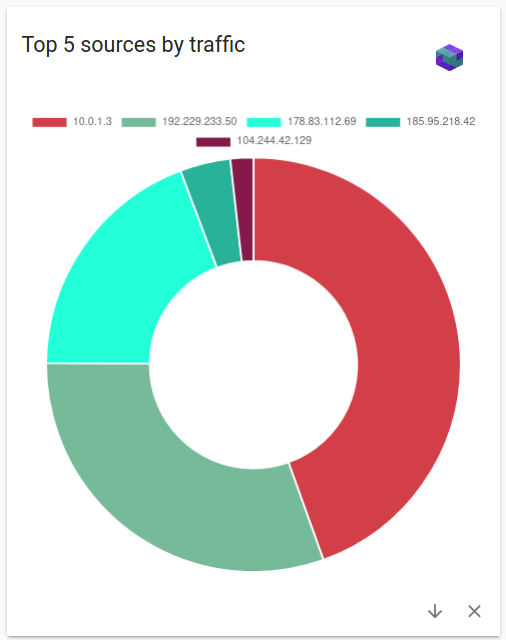
\includegraphics[width=10cm]{images/researcher-case-study-first-result.png}
    \caption{Plotting a dataset using the first version of the feature miner}
    \label{fig:firstimplementation}
\end{figure}

As one might have noticed there has been no asynchronous logic in the method that is called once the decoding has finished. This will now become important since the researcher would like to supplement the current result with data from a remote WHOIS database. We will not go into detail about how the IP lookup using the WHOIS protocol works but we will show how one can perform asynchronous operations in this part of the lifecycle to enrich the data.
To implement the lookups of the source addresses the labels of the diagram need to be reformatted to include the desired information. The researcher thus changes the \textit{formatLabels} method as shown in listing \ref{lst:formatlabels} so that it fetches the WHOIS data and returns that for labelling.

\begin{lstlisting}[caption={Initial content of the newly create Miner},float=H,label={lst:formatlabels}]
    // ...
    
    async formatLabels (elements) {
        var addresses = elements.map(entry => entry.addr)
        var result = []
        for(var address of addresses) {
            var { route, origin, country } = await this.whois(address)
            
            // Format example: 1.2.3.4: 1.2.0.0/16 (AS12345, CH)
            var label = `${address}: ${route} (${origin}, ${country})`
            result.push(label)
        }
        return result
    }
    
    // ...
\end{lstlisting}
The implementation of that method is straightforward, the researcher makes sure that the corresponding prefix, origin AS number and country are retrieved form the WHOIS service. These elements are used along with the source address to create a label for the diagram.
Now, the researcher can use any dataset found in a database such as DDoSDB.org and derive the additional information using our tool. This final visualization is shown in figure \ref{fig:finalimpl}

\begin{figure}[]
    \centering
    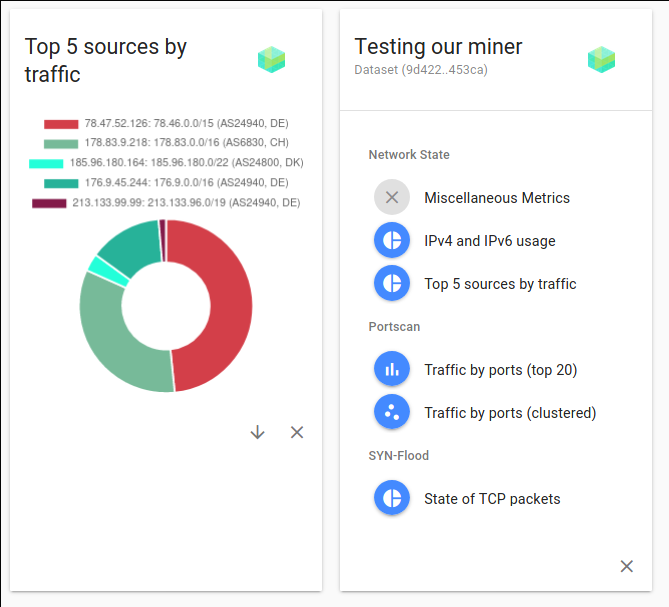
\includegraphics[width=15cm]{images/reseracher-case-study-final.png}
    \caption{Final visualization once the supplemental data has been integrated}
    \label{fig:finalimpl}
\end{figure}

As we saw in the previous paragraphs the researcher was able to compute and visualize new information from his PCAP file and even integrate other data sources.
We think it is important to note that only the newly created file had to be touched. It was not necessary to modify other feature miners, orchestration modules or the front-end. Thus it is possible to extend the functionality without modifying existing functionality.

\section{Future Work} % MF: Discussion and Limitations? Add related work together with conclusions as one paragraph
This paper describes the implementation of a general-purpose DDoS visualization system. It has been implemented requirements in mind such as agnositicity to scale and type of attack and the software and location of network capture.
The prototypical implementation has covered visualizations such as x, y, z (??) and used a PCAP files as a data source.
The architecture and design of the system have been written with extensibility in mind, which should allow that the following subsystems of the solution could easily be adapted, exchanged or extended:
\begin{itemize}

    \item Data source: The application was targeted to use PCAP files, since they are the most common in DDoSDB, a collection of network attacks. A common format that enables similar insights into network traffic flow is NetFlow. In the analysis of possible data sets we found that NetFlow files could also be used as a data source. By complying with the systems architecture consisting of interfaces and a Visitor pattern one could provide an alternate, Netflow-based data source parser.
    
    \item Data pre-processing: The implementation can be used with network logs from DDoSDB, which are already anonymised. If a raw packet capture is supplied the same pre-processing is applied. Given certain constraints such as data privacy laws, this part could be easily extended.
    
    \item Data processing / parsing:
    Creating new analysis processors for the existing PCAP-files would be very easy to write. The user would simply have to register a new visitor and comply with the interfaces or extend them for novel visualizations. For example, assuming that a new application-level protocol would be targeted, the visitor can be registered to be invoked for those types of packets and compute his metrics.
   
    \item Data integration:
    The system is not integrated with DDoSDB in a fully automated manner due to lack of interfaces. Technically, it would be possible to integrate the uploading  of processed files to DDoSDB or the download such files.
    
    \item Visualizations
    The part that is easiest to adapt and extend is the set of visualizations. Since the front-end was written with a component-based approach one can easily reuse and change the visualizations. By adhering to the dataset a developer can easily create new components and integrate them into the system without having to know all too much about the systems internals, such as the data processing.
\end{itemize}